\documentclass[10pt,a4paper]{article}

\usepackage{preambule}
\fancyhead[L]{\scriptsize \textsc{Nora NICOLAS}}
\fancyhead[R]{\scriptsize \textsc{Contrôle d'électricité numéro 1, S1 GC, sujet
1}}

\setlength{\parindent}{0pt}

\titleformat{\section}{\color{blue}\bfseries\Large}{Exercice \Roman{section})
}{.0em}{}{}
\titleformat{\subsection}[runin]{\color{brandeisblue}\bfseries\large}
{\Roman{section})\hspace{.5em}\arabic{subsection}-}{.5em}{}{}
\titleformat{\subsubsection}{\color{capri}\bfseries}{\Roman{section})
\arabic{subsection}- \alph{subsubsection}.}{.5em}{}{}

\begin{document}

\noindent \Ul{Nom} : \hfill \Ul{Prénom} : \hfill \Ul{Date} : \hfill \Ul{Note} :
\hspace*{3em}\bigbreak

Tout oubli d’unité ou de chiffres significatifs pourra entraîner la perte de
point, même si la réponse est juste. \Ul{Un schéma est systématiquement
nécessaire}. Les détails des calculs sont nécessaires. Une expression littérale
est attendue avant toute application numérique. Pensez à respecter la notation
de l'énoncé.

\section{Résistance équivalente}
Calculez la résistance équivalente de l'association suivante.
\begin{figure}[htbp!]
    \centering
    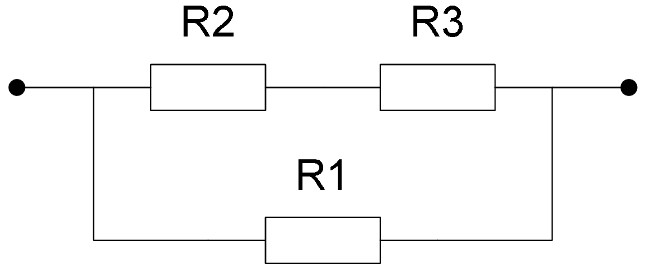
\includegraphics[width=.3\linewidth]{Req1.png}
    \captionsetup{justification=centering}
\end{figure}

On donne $R_1 = \SI{330}{\O}$, $R_2 = \SI{220}{\O}$ et $R_3 = \SI{820}{\O}$.

\vfill

\section{Conventions}
\noindent On constitue un circuit électrique avec un générateur réel de tension
$(E, r)$, entre les bornes duquel on branche une résistance $R$.

\subsection{}Fléchez chaque dipôle en convention récepteur.
\vspace{3cm}
\subsection{}Fléchez chaque dipôle en convention générateur.
\vspace{3cm}
\subsection{}Fléchez chaque dipôle en fonction de sa nature, et déterminez
l'intensité parcourant le circuit.
\vspace{3cm}

\newpage

\section{Diviseur de tension}
\begin{wrapfigure}[3]{R}{.2\linewidth}
    \centering
    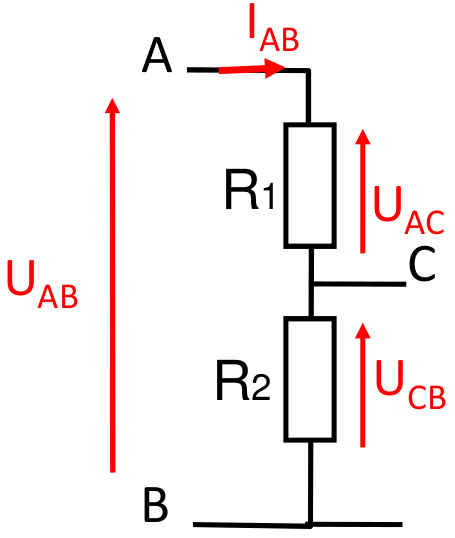
\includegraphics[width=\linewidth]{DivTen.png}
    \captionsetup{justification=centering}
\end{wrapfigure}
Exprimez (et détaillez le calcul) la tension $U\St{CB}$ en fonction de
$U\St{AB}$, $R_1$ et $R_2$.

\vfill

\section{Calcul de courants}
Calculez $I_1$, $I_2$ et $I_3$.
\begin{figure}[htbp!]
    \centering
    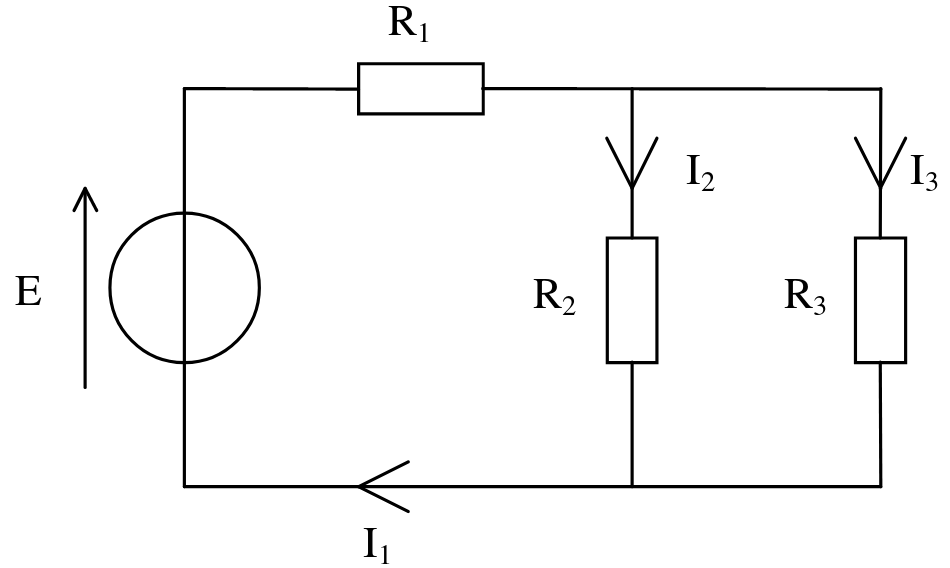
\includegraphics[width=.4\linewidth]{Courants.png}
    \captionsetup{justification=centering}
\end{figure}

On donne : $E = \SI{6}{V}$, $R_1 = \SI{270}{\O}$, $R_2 = \SI{470}{\O}$ et $R_3 =
\SI{220}{\O}$.

\vspace{12cm}

\end{document}
